\chapter{算术逻辑运算单元ALU设计实验}
\section{实验内容}

设计算术逻辑运算单元 ALU。

\section{实验原理}

\begin{figure}[H]
\centering
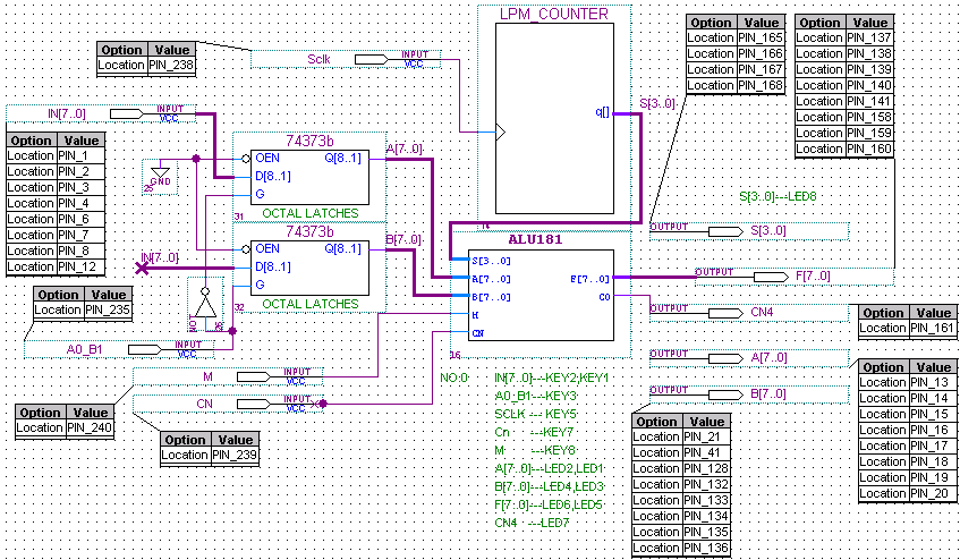
\includegraphics[width=\textwidth]{images/prin3.png}
\caption{ALU 实验原理图}
\label{fig:prin3}
\end{figure}

如图\ref{fig:prin3},由74LS181 (ALU 181), LPM\_COUNTER, 两个 74383b 锁存器, 非门组成,数据线 8 位。

\subsubsection{输入信号}

\begin{itemize}
    \item Sclk
    
    时钟信号。

    可由外部控制的输入信号。
    
    \item IN[7..0]
    
    数据信号,8 位,用于输入源操作数。
    
    可由外部控制的输入信号。
    
    \item A0\_B1
    
    片选信号,控制源操作数进入不同的锁存器。
    
    可由外部控制的输入信号。
    
    \item M
    
    运算模式控制。0: 算术运算, 1: 逻辑运算。
    
    可由外部控制的输入信号。
    
    \item CN
    
    运算模式控制。0: 无进位, 1: 带进位。
    
    可由外部控制的输入信号。
    
\end{itemize} 

\subsubsection{输出信号}

\begin{itemize}
    \item S[3..0]
    
    ALU 功能码,4 位。
    
    \item F[7..0]
    
    ALU 输出,8 位。
    
    \item CN4
    
    进位标记。
    
    \item A[7..0]
    
    输出源操作数 A 的值,8 位。
    
    \item B[7..0]
    
    输出源操作数 B 的值,8 位。
    
\end{itemize}

\section{实验任务与实验步骤}

\begin{enumerate}
    \item 按照原理图 \ref{fig:prin3} 连接电路图,然后编译。
    
    \begin{enumerate}
        \item 用 VDHL 语言对 74LS181 编程。
        
        \lstinputlisting[language=VHDL, caption={alu181.vhd}, label={code:alu181}]{codes/alu181.vhd}
    \end{enumerate}
    
    \item 将输入输出器件绑定到对应的引脚上,然后重新编译。
    
    \begin{table}[H]
        \centering
        \begin{tabular}{|c|c|c|}
            \hline
            名称 & 引脚号 & 备注 \\
            \hline
            A0\_B1 & 235 & Key 3 \\
            \hline
            Sclk & 238 & Key 6 \\
            \hline
            CN & 239 & Key 7 \\
            \hline
            M & 240 & Key 8 \\
            \hline
            IN[0] & 1 & Key 1 \\
            \hline
            IN[1] & 2 & Key 1 \\
            \hline
            IN[2] & 3 & Key 1 \\
            \hline
            IN[3] & 4 & Key 1 \\
            \hline
            IN[4] & 6 & Key 2 \\
            \hline
            IN[5] & 7 & Key 2 \\
            \hline
            IN[6] & 8 & Key 2 \\
            \hline
            IN[7] & 12 & Key 2 \\
            \hline
            A[0] & 13 & 数码 1 \\
            \hline
            A[1] & 14 & 数码 1 \\
            \hline
            A[2] & 15 & 数码 1 \\
            \hline
            A[3] & 16 & 数码 1 \\
            \hline
            A[4] & 17 & 数码 2 \\
            \hline
            A[5] & 18 & 数码 2 \\
            \hline
            A[6] & 19 & 数码 2 \\
            \hline
            A[7] & 20 & 数码 2 \\
            \hline
            B[0] & 21 & 数码 3 \\
            \hline
            B[1] & 41 & 数码 3 \\
            \hline
            B[2] & 128 & 数码 3 \\
            \hline
            B[3] & 132 & 数码 3 \\
            \hline
            B[4] & 133 & 数码 4 \\
            \hline
            B[5] & 134 & 数码 4 \\
            \hline
            B[6] & 135 & 数码 4 \\
            \hline
            B[7] & 136 & 数码 4 \\
            \hline
            F[0] & 137 & 数码 5 \\
            \hline
            F[1] & 138 & 数码 5 \\
            \hline
            F[2] & 139 & 数码 5 \\
            \hline
            F[3] & 140 & 数码 5 \\
            \hline
            F[4] & 141 & 数码 6 \\
            \hline
            F[5] & 158 & 数码 6 \\
            \hline
            F[6] & 159 & 数码 6 \\
            \hline
            F[7] & 160 & 数码 6 \\
            \hline
            CN & 161 & 数码 7 \\
            \hline
            S[0] & 165 & 数码 8 \\
            \hline
            S[1] & 166 & 数码 8 \\
            \hline
            S[2] & 167 & 数码 8 \\
            \hline
            S[3] & 168 & 数码 8 \\
            \hline
        \end{tabular}
        \caption{ALU 实验引脚表}
        \label{tab:pin3}
    \end{table}
    
    
    \item 下载到实验设备上。
    \item 调整为工作模式 0。
    \item 观察实验现象。
    
    \begin{itemize}
        \item Key 1, 2 (D1 - D8)
        
        控制输入数据,8 位全有效,同时根据 A0\_B1 的值显示在数码 1 - 2 或数码 3 - 4 上。
        
        \item Key 3 (D11)
        
        控制当前输入的是第一个源操作数还是第二个源操作数,锁定 A0\_B1 的值。
        
        \item Key 6 (D14)
        
        控制时钟。其值通过 LPM\_COUNTER 累加器反映到数码 8 上。
        
        \item Key 7
        
        控制 CN 输入,影响 ALU,切换(带/无)进位运算模式。
        
        \item Key 8
        
        控制 M 输入,影响 ALU,切换(逻辑/算数)运算模式。
        
        \item 数码管 1, 2
        
        第一个源操作数,8 位全有效。
        
        \item 数码管 3, 4
        
        第二个源操作数,8 位全有效。
        
        \item 数码管 5, 6
        
        ALU 计算结果,8 位全有效。
        
        \item 数码管 7
        
        ALU 计算结果的进位标记位,最低位有效。
        
        \item 数码管 8
        
        ALU 功能码,4 位全有效。
        
    \end{itemize}
    \item 绘制仿真波形图。
\end{enumerate}

\section{实验结果分析}

\subsection{实验电路图}

根据原理图 \ref{fig:prin3} 绘制实验电路图 \ref{fig:bdf3}。

\begin{figure}[H]
\centering
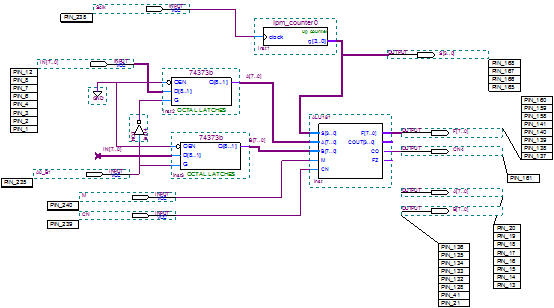
\includegraphics[width=\textwidth]{images/bdf3.png}
\caption{ALU 实验电路图}
\label{fig:bdf3}
\end{figure}

\subsection{仿真波形图}

利用 Quartus II 产生仿真波形图 \ref{fig:wave3_1},\ref{fig:wave3_2}。

\begin{figure}[H]
\centering
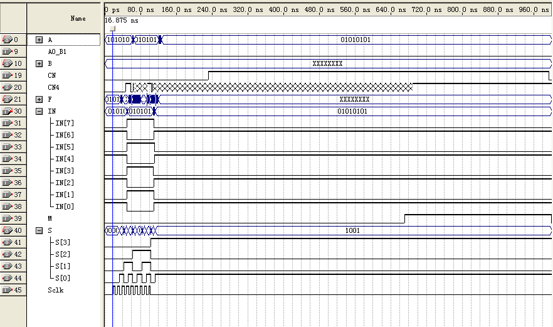
\includegraphics[width=\textwidth]{images/wave3_1.png}
\caption{ALU 实验 仿真波形图 1}
\label{fig:wave3_1}
\end{figure}

\begin{figure}[H]
\centering
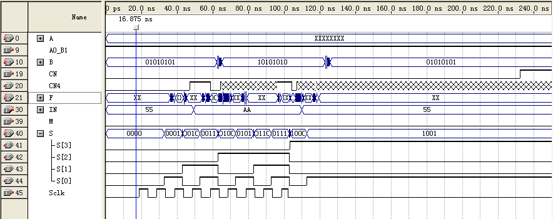
\includegraphics[width=\textwidth]{images/wave3_2.png}
\caption{ALU 实验 仿真波形图 2}
\label{fig:wave3_2}
\end{figure}


\subsection{附加题}

\begin{enumerate}
    \item 完成真值表:
    
    \textbf{答}:
    
    实验所得真值表如下:
    
    \begin{table}[H]
        \centering
        \begin{tabular}{|c c c c|c c|c c|c|c|c|}
            \hline
            \multicolumn{4}{|c|}{S[4..0]} & \multicolumn{2}{c|}{A[7..0]} & \multicolumn{2}{c}{B[7..0]} & \multicolumn{2}{|c|}{算术运算 M = 0} & 逻辑运算 M = 1 \\
            \hline
            S3 & S2 & S1 & S0 & AH & AL & BH & BL & CN = 0 (无进位) & CN = 1 (有进位) & \\
            \hline
            0 & 0 & 0 & 0 & A & A & 5 & 5 & 0AA & 0AB & \cellcolor[HTML]{FFF9C4}155 \\
            \hline
            0 & 0 & 0 & 1 & A & A & 5 & 5 & 0FF & 100 & \cellcolor[HTML]{FFF9C4}100 \\
            \hline
            0 & 0 & 1 & 0 & A & A & 5 & 5 & \cellcolor[HTML]{FFF9C4}1AA & \cellcolor[HTML]{FFF9C4}1AB & 055 \\
            \hline
            0 & 0 & 1 & 1 & A & A & 5 & 5 & 0FF & \cellcolor[HTML]{FFF9C4}1FF & 000 \\
            \hline
            0 & 1 & 0 & 0 & F & F & 0 & 1 & 1FD & 1FE & \cellcolor[HTML]{FFF9C4}1FE \\
            \hline
            0 & 1 & 0 & 1 & F & F & 0 & 1 & 1FD & 1FE & \cellcolor[HTML]{FFF9C4}1FE \\
            \hline
            0 & 1 & 1 & 0 & F & F & 0 & 1 & 0FE & 0FD & 0FE \\
            \hline
            0 & 1 & 1 & 1 & F & F & 0 & 1 & \cellcolor[HTML]{FFF9C4}1FF & \cellcolor[HTML]{FFF9C4}1FE & 0FE \\
            \hline
            1 & 0 & 0 & 0 & F & F & 0 & 1 & 100 & 101 & \cellcolor[HTML]{FFF9C4}101 \\
            \hline
            1 & 0 & 0 & 1 & F & F & 0 & 1 & 100 & 101 & \cellcolor[HTML]{FFF9C4}101 \\
            \hline
            1 & 0 & 1 & 0 & F & F & 0 & 1 & \cellcolor[HTML]{FFF9C4}000 & \cellcolor[HTML]{FFF9C4}001 & 001 \\
            \hline
            1 & 0 & 1 & 1 & F & F & 0 & 1 & 001 & 000 & 000 \\
            \hline
            1 & 1 & 0 & 0 & F & F & 0 & 1 & 1FE & 1FF & 001 \\
            \hline
            1 & 1 & 0 & 1 & 5 & 5 & 0 & 1 & 0AA & 0AB & \cellcolor[HTML]{FFF9C4}1FF \\
            \hline
            1 & 1 & 1 & 0 & 5 & 5 & 0 & 1 & \cellcolor[HTML]{FFF9C4}054 & \cellcolor[HTML]{FFF9C4}055 & 055 \\
            \hline
            1 & 1 & 1 & 1 & 5 & 5 & 0 & 1 & 055 & 054 & 055 \\
            \hline
        \end{tabular}
        \caption{ALU 实验值}
        \label{tab:addi3_1}
    \end{table}
    
    理论值表计算如下,两个表中标记黄色的单元格为实验值与理论值不同之处。
    
    \begin{table}[H]
        \centering
        \begin{tabular}{|c c c c|c c|c c|c|c|c|}
            \hline
            \multicolumn{4}{|c|}{S[4..0]} & \multicolumn{2}{c|}{A[7..0]} & \multicolumn{2}{c}{B[7..0]} & \multicolumn{2}{|c|}{算术运算 M = 0} & 逻辑运算 M = 1 \\
            \hline
            S3 & S2 & S1 & S0 & AH & AL & BH & BL & CN = 0 (无进位) & CN = 1 (有进位) & \\
            \hline
            0 & 0 & 0 & 0 & A & A & 5 & 5 & 0AA & 0AB & \cellcolor[HTML]{FFF9C4}055 \\
            \hline
            0 & 0 & 0 & 1 & A & A & 5 & 5 & 0FF & 100 & \cellcolor[HTML]{FFF9C4}000 \\
            \hline
            0 & 0 & 1 & 0 & A & A & 5 & 5 & \cellcolor[HTML]{FFF9C4}0AA & \cellcolor[HTML]{FFF9C4}0AB & 055 \\
            \hline
            0 & 0 & 1 & 1 & A & A & 5 & 5 & 0FF & \cellcolor[HTML]{FFF9C4}0FF & 000 \\
            \hline
            0 & 1 & 0 & 0 & F & F & 0 & 1 & 1FD & 1FE & \cellcolor[HTML]{FFF9C4}0FE \\
            \hline
            0 & 1 & 0 & 1 & F & F & 0 & 1 & 1FD & 1FE & \cellcolor[HTML]{FFF9C4}0FE \\
            \hline
            0 & 1 & 1 & 0 & F & F & 0 & 1 & 0FE & 0FD & 0FE \\
            \hline
            0 & 1 & 1 & 1 & F & F & 0 & 1 & \cellcolor[HTML]{FFF9C4}0FF & \cellcolor[HTML]{FFF9C4}0FE & 0FE \\
            \hline
            1 & 0 & 0 & 0 & F & F & 0 & 1 & 100 & 101 & \cellcolor[HTML]{FFF9C4}001 \\
            \hline
            1 & 0 & 0 & 1 & F & F & 0 & 1 & 100 & 101 & \cellcolor[HTML]{FFF9C4}001 \\
            \hline
            1 & 0 & 1 & 0 & F & F & 0 & 1 & \cellcolor[HTML]{FFF9C4}100 & \cellcolor[HTML]{FFF9C4}101 & 001 \\
            \hline
            1 & 0 & 1 & 1 & F & F & 0 & 1 & 001 & 000 & 000 \\
            \hline
            1 & 1 & 0 & 0 & F & F & 0 & 1 & 1FE & 1FF & 001 \\
            \hline
            1 & 1 & 0 & 1 & 5 & 5 & 0 & 1 & 0AA & 0AB & \cellcolor[HTML]{FFF9C4}0FF \\
            \hline
            1 & 1 & 1 & 0 & 5 & 5 & 0 & 1 & \cellcolor[HTML]{FFF9C4}154 & \cellcolor[HTML]{FFF9C4}155 & 055 \\
            \hline
            1 & 1 & 1 & 1 & 5 & 5 & 0 & 1 & 055 & 054 & 055 \\
            \hline
        \end{tabular}
        \caption{ALU 理论值}
        \label{tab:addi3_2}
    \end{table}
    
    发现偏差都表现在进位位上,分析原因发现 VHDL 代码 \ref{code:alu181} 中关于进位位的实现有问题。
    
\end{enumerate}
